\documentclass[11pt]{article}
\usepackage[margin=1in]{geometry}
\usepackage{amsmath,amssymb,amsthm}
\usepackage{booktabs}
\usepackage{enumitem}
\usepackage{tikz}
\usetikzlibrary{arrows.meta}
\usepackage[most]{tcolorbox}
\usepackage{hyperref}
\hypersetup{colorlinks=true,linkcolor=blue,urlcolor=blue}

\theoremstyle{plain}
\newtheorem{theorem}{Theorem}[section]
\newtheorem{lemma}[theorem]{Lemma}
\newtheorem{conjecture}[theorem]{Conjecture}
\theoremstyle{definition}
\newtheorem{definition}[theorem]{Definition}
\newtcolorbox{ponder}{colback=yellow!6,colframe=orange!60!black,boxrule=0.5pt,
  left=4pt,right=4pt,top=2pt,bottom=2pt,fonttitle=\bfseries\small,title=Ponder}
\newtcolorbox{status}{colback=blue!4,colframe=blue!50!black,boxrule=0.5pt,
  left=4pt,right=4pt,top=2pt,bottom=2pt,fonttitle=\bfseries\small,title=Status}
\setlength{\parskip}{0.45em}\setlength{\parindent}{0pt}
\newcommand{\T}{\square}

\title{3-Choosability of Toroidal Grids:\\ the Problem, the Solved Cases, and Where We Are}
\author{Reference document for Sid}
\date{October 26, 2026}

\begin{document}
\maketitle
\tableofcontents
\bigskip

\section{The problem}

\paragraph{List colouring.} A \emph{list assignment} $L$ gives each vertex $v$ a set $L(v)$
of allowed colours. $G$ is \emph{$L$-colourable} if there is a proper colouring with
$c(v)\in L(v)$ for all $v$. $G$ is \emph{$k$-choosable} if it is $L$-colourable whenever
every $|L(v)|\ge k$. The smallest such $k$ is the \emph{choice number} $\chi_\ell(G)$.
Always $\chi(G)\le\chi_\ell(G)$, and the gap can be large: $K_{n,n}$ is 2-colourable but its
choice number grows with $n$. So knowing $G$ is 3-colourable says little about lists.

\paragraph{The graph.} The toroidal grid $C_m\T C_n$ has vertices $(r,c)$, $r\in\mathbb Z_m$
(row), $c\in\mathbb Z_n$ (column). $(r,c)$ is adjacent to $(r\pm1,c)$ (\emph{column edges}:
each column is a copy of $C_m$) and $(r,c\pm1)$ (\emph{row edges}: each row is a copy of
$C_n$). It is 4-regular, so greedy colouring gives 5-choosable, and it is 3-colourable for
all $m,n\ge3$.

\begin{figure}[ht]\centering
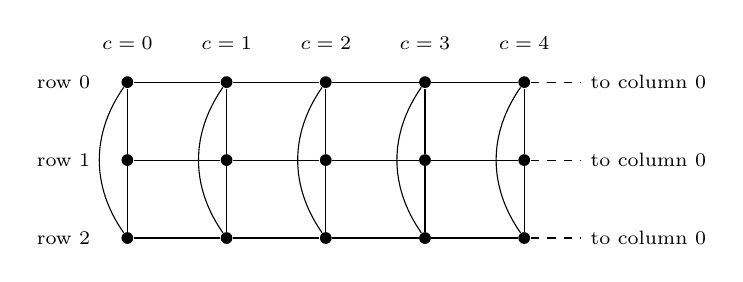
\begin{tikzpicture}[v/.style={circle,fill=black,inner sep=1.5pt},scale=0.9]
\foreach \c in {0,...,4}{\foreach \r in {0,1,2}{\node[v] (v\r\c) at (\c*1.4,-\r*1.1) {};}}
\foreach \c in {0,...,4}{\draw (v0\c)--(v1\c)--(v2\c); \draw (v0\c) to[bend right=35] (v2\c);}
\foreach \r in {0,1,2}{\foreach \c/\d in {0/1,1/2,2/3,3/4}{\draw (v\r\c)--(v\r\d);}
  \draw[dashed] (v\r4)--++(0.8,0) node[right,font=\scriptsize]{to column 0};}
\foreach \c in {0,...,4}{\node[font=\scriptsize] at (\c*1.4,0.55) {$c=\c$};}
\foreach \r in {0,1,2}{\node[font=\scriptsize] at (-0.9,-\r*1.1) {row \r};}
\end{tikzpicture}
\caption{$C_3\T C_5$: each column is a triangle, each row a 5-cycle (dashed edges wrap around).}
\end{figure}

\begin{conjecture}[Cai, Wang, Zhu, 2010]
Every toroidal grid $C_m\T C_n$ ($m,n\ge3$) is 3-choosable.
\end{conjecture}

Split by parity of $m,n$:
\begin{center}
\begin{tabular}{@{}lll@{}}
\toprule
case & status & by \\
\midrule
both even & 3-choosable & Alon--Tarsi, easy (bipartite)\\
one odd, one even & 3-choosable & Alon--Tarsi, Li--Shao--Petrov--Gordeev 2023\\
$m=3$, $n$ odd & 3-choosable (claimed) & Galvin for $n=3$; your partner for all odd $n$\\
both odd, $m,n\ge5$ & \textbf{open} & this is the target\\
\bottomrule
\end{tabular}
\end{center}

\section{The main tool: Alon--Tarsi}

\paragraph{Graph polynomial.} Orient each edge $uv$ as $u\to v$ and put
$P_G=\prod_{u\to v}(x_u-x_v)$. A colouring $c$ is proper iff $P_G(c)\ne0$.

\begin{lemma}[Combinatorial Nullstellensatz]
If $\deg P=\sum_v t_v$ and the coefficient of $\prod_v x_v^{t_v}$ in $P$ is nonzero, then for
any sets $S_v$ with $|S_v|>t_v$ there are $s_v\in S_v$ with $P(s)\ne0$.
\end{lemma}

So if $[\prod x_v^{t_v}]P_G\ne0$, then $G$ is colourable from any lists with
$|L(v)|\ge t_v+1$. The \emph{Alon--Tarsi number} $AT(G)$ is the least $k$ such that some
monomial with all $t_v\le k-1$ has nonzero coefficient. Always $\chi_\ell\le AT$.

\paragraph{Key simplification for our graphs.} $C_m\T C_n$ has $N=mn$ vertices and $2N$
edges, so $\deg P_G=2N$. A monomial with every $t_v\le2$ and total degree $2N$ must be
$\prod_v x_v^2$. Hence
\[
AT(C_m\T C_n)\le 3 \iff [\textstyle\prod_v x_v^2]\,P_G\ne0 .
\]
Combinatorially, this coefficient equals $\pm(EE-EO)$ for an orientation with all
out-degrees $2$, where $EE$/$EO$ count spanning Eulerian subgraphs with an even/odd number
of edges (the Alon--Tarsi theorem).

\subsection*{Case 1: both even}
$G$ is bipartite, so every cycle, hence every Eulerian subgraph, has an even number of
edges: $EO=0$ and $EE\ge1$ (the empty subgraph). Take any Eulerian orientation (all
out-degrees 2, exists since $G$ is 4-regular). So $AT\le3$, and $G$ is 3-choosable.

\subsection*{Case 2: one odd, one even}
Not bipartite, so the counting is no longer trivial. Li--Shao--Petrov--Gordeev computed the
coefficient with the \emph{coefficient formula} below and showed it is nonzero. Same
conclusion: $AT=3$.

\begin{lemma}[Laso\'n; Karasev--Petrov]
If $\deg Q\le\sum t_v$ and $|A_v|=t_v+1$, then
\[
[\textstyle\prod x_v^{t_v}]\,Q=\sum_{\varphi\in\prod A_v}\dfrac{Q(\varphi)}{\prod_v N_v(\varphi(v))},
\qquad N_v(a)=\prod_{b\in A_v,b\ne a}(a-b).
\]
\end{lemma}

Choosing every $A_v=\{1,\omega,\omega^2\}$ (cube roots of unity) turns the coefficient into a
sum over \emph{3-colourings with colours $1,\omega,\omega^2$}, weighted by products of
differences. On a grid this sum factorises column by column: a \emph{transfer matrix}
$T$ indexed by colourings of one column, and the coefficient is $\operatorname{tr}(T^n)$.

\subsection*{Why both odd is different}
Li--Shao--Petrov--Gordeev also proved $AT=4$ when $m,n$ are both odd: the coefficient of
$\prod x_v^2$ is exactly $0$. Your partner reproved this for $m=3$ in two lines: the
nonzero eigenvalues of $T$ come in pairs $\pm\lambda$ ($\pm i\sqrt3$), so
$\operatorname{tr}(T^n)=\sum(\lambda^n+(-\lambda)^n)=0$ for odd $n$.

\begin{ponder}
Why does the $\pm$ pairing of eigenvalues kill the trace exactly for odd $n$? Which symmetry
of the column states (he calls them even/odd states) produces the pairing?
\end{ponder}

So for odd $\times$ odd, Alon--Tarsi cannot work: any proof must be genuinely about
lists, not about one polynomial coefficient.

\section{Case 3: \texorpdfstring{$m=3$}{m = 3}, \texorpdfstring{$n$}{n} odd}

\subsection{$n=3$: Galvin}
$C_3\T C_3=K_3\T K_3$ is the line graph of $K_{3,3}$ (cells of a $3\times3$ grid, adjacent if
in the same row or column). Galvin's theorem (the Dinitz conjecture proof) gives
3-choosability. Galvin's method is the \emph{kernel method}, which reappears in
Section~5.

\subsection{Your partner's route, step by step}

His work came in three stages: an Alon--Tarsi result on a damaged graph, a full
(partly computer-checked) proof in his paper [P], then a computer-free proof (the
October 20 note). The ideas, in the order he found them:

\paragraph{Step 1: what is \emph{almost} true? Delete one edge.}
For $G$ the coefficient is $0$. Delete one edge $e$: $G-e$ has $2N-1$ edges, so the natural
monomial is $x_w\prod_{v\ne w}x_v^2$ (one vertex $w$ gets exponent 1).

\begin{theorem}[Partner, ``Deleting one edge\ldots'']
For odd $n$, every edge $e$ and every $w$ not on the cycle (column triangle or row cycle)
through $e$: $c_w=[x_w\prod_{v\ne w}x_v^2]P_{G-e}\ne0$, with an exact formula (powers of 3).
\end{theorem}

\emph{How:} the coefficient formula with cube roots of unity. In an undamaged column a
contributing colouring is a permutation of $(1,\omega,\omega^2)$: 6 \emph{states}. The
transfer matrix is $T=\sigma(S^2-S)$ ($S$: multiply the state by $\omega$; $\sigma$: $\pm1$
on even/odd permutations), so $T^3=-3T$ and everything diagonalises in closed form. The
damaged column (12 contributing triples) breaks the $\pm$ symmetry, and the factor
$\varphi(w)$ at $w$ shifts the eigen-mode; summing gives nonzero powers of $3$.

\emph{Consequences:}
\begin{itemize}[nosep]
\item $G-e$ is 3-choosable, even with $|L(w)|=2$.
\item \textbf{If some edge $uv$ of $G$ has $L(u)\cap L(v)=\emptyset$, $G$ is $L$-colourable}
(colour $G-e$; the edge $uv$ is automatically fine).
\end{itemize}
So a bad list assignment must have overlapping lists on \emph{every} edge. This is the
first structural restriction on a counterexample.

\begin{ponder}
Why must $w$ be off the cycle of $e$? (For a row edge, $w$ in that row gives
$\beta_0=\omega^0-\omega^0=0$.) What does that say about which vertex can have the short list?
\end{ponder}

\paragraph{Step 2: the strip lemma (pinning colours at the ends).}
Cut the torus open: $H_m=C_3\T P_m$ (a strip of $m$ columns). An \emph{end multiset} $S$ picks
three vertices in the first and last columns with multiplicity $\le2$; let $k$ be how many
lie in the last column and $s=\sum\mu_S(v)\,\mathrm{row}(v)\bmod3$.

\begin{theorem}[Odd strip lemma]
For odd $m\ge3$, $1\le k\le2$ and $s\not\equiv0$: $c_S\ne0$, where
$c_S=-\tfrac g9\mu_k^{m-1}(\omega^s-\omega^{2s})$. Hence $H_m$ is $L$-colourable whenever
$|L(v)|\ge 3-\mu_S(v)$.
\end{theorem}
Meaning: you may \emph{fix} a colour at a vertex of multiplicity 2 (list of size 1) and
\emph{forbid} a colour at a vertex of multiplicity 1 (list of size 2), and the strip is still
colourable. This is the tool for gluing.

\begin{ponder}
Where exactly does $s\not\equiv0\pmod3$ come from, and why does the formula use
$(-1)^m$ so that odd $m$ matters? (For even $m$ the bracket is $\omega^s+\omega^{2s}$.)
\end{ponder}

\paragraph{Step 3: the prism lemma (exact obstruction for two columns).}
The prism is two triangles $U=u_0u_1u_2$, $V=v_0v_1v_2$ joined by $u_tv_t$.

\begin{lemma}[Prism lemma]
Let $|L(u_0)|\ge3$ and $|L(w)|\ge2$ elsewhere. $P$ is not $L$-colourable iff
\textbf{(Z)} $L(v_0)=L(v_1)=L(v_2)$ is one 2-set, or
\textbf{(W)} $L(u_1)=L(u_2)=D$, $L(u_0)=D\cup\{\zeta\}$, $L(v_1)=L(v_2)=E$ and
$L(v_0)\setminus E=\{\zeta\}$ ($D,E$ 2-sets).
\end{lemma}
In (W), $u_1,u_2$ use up $D$, forcing $u_0=\zeta$; $v_1,v_2$ use up $E$, forcing $v_0=\zeta$:
conflict. The proof is Hall's theorem on triangles plus case analysis.

\begin{figure}[ht]\centering
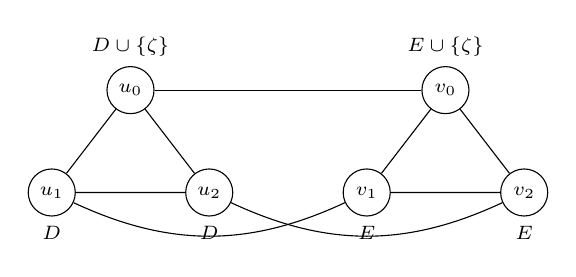
\begin{tikzpicture}[v/.style={circle,draw,minimum size=17pt,inner sep=0pt,font=\scriptsize},scale=1]
\node[v] (u0) at (0,0) {$u_0$}; \node[v] (u1) at (-1,-1.3) {$u_1$}; \node[v] (u2) at (1,-1.3) {$u_2$};
\node[v] (v0) at (4,0) {$v_0$}; \node[v] (v1) at (3,-1.3) {$v_1$}; \node[v] (v2) at (5,-1.3) {$v_2$};
\draw (u0)--(u1)--(u2)--(u0); \draw (v0)--(v1)--(v2)--(v0);
\draw (u0)--(v0); \draw (u1) to[bend right=25] (v1); \draw (u2) to[bend right=25] (v2);
\node[font=\scriptsize,above] at (u0.north) {$D\cup\{\zeta\}$};
\node[font=\scriptsize,below] at (u1.south) {$D$}; \node[font=\scriptsize,below] at (u2.south) {$D$};
\node[font=\scriptsize,above] at (v0.north) {$E\cup\{\zeta\}$};
\node[font=\scriptsize,below] at (v1.south) {$E$}; \node[font=\scriptsize,below] at (v2.south) {$E$};
\end{tikzpicture}
\caption{Configuration (W): both triangles are forced to put $\zeta$ on the edge $u_0v_0$.}
\end{figure}

\textbf{Two-column extension} (corollary): given fixed colours on the left of column $M$ and
on the right of column $N$, if $M,N$ cannot be filled then $|L_N(r')\cap L_N(r'')|=2$ and the
colour forced at $(r',N)$ is the unique colour of $L_N(r')\setminus L_N(r'')$. So failure is
predictable, and can be dodged in advance.

\paragraph{Step 4: the propagation lemma (from [P]).}
Let $F(c)=L(0,c)\cap L(1,c)\cap L(2,c)$, the colours common to column $c$. For any list
assignment with no colouring (lists of size exactly 3):
\[
L(r,c)\setminus F(c)\subseteq L(r,c+1)\qquad\text{for all } r,c. \tag{$\ast$}
\]
\begin{status}
This is [P, Lemma 3.5]. We have not seen its proof. It rests on further lemmas of [P] and on
the column-edge case of the edge-deletion theorem. Everything else in the proof is in the notes
we have.
\end{status}

\paragraph{Step 5: the proof.} Suppose $L$ (all lists of size 3, $n\ge5$ odd) has no colouring.

\emph{Case A: $F(j)\not\subseteq F(j+1)$ for some $j$.} Take $\alpha\in F(j)\setminus F(j+1)$
and a row $r$ with $\alpha\notin L(r,j+1)$. Name columns $C_0,\dots,C_3=j,\dots,j+3$. Delete
$C_1,C_2$: what remains is a strip of $n-2$ columns (odd) from $C_3$ around to $C_0$. Use the
strip lemma with $S=\{(r,C_0),(r,C_0),(r',C_3)\}$: fix $(r,C_0)=\alpha$ and forbid a
cleverly chosen $\beta$ at $(r',C_3)$ ($s=2r+r'\equiv r'-r\not\equiv0$). Now fill $C_1,C_2$.
Row $r$ is automatically fine since $\alpha\notin L(r,C_1)$. The two-column lemma says the
only way to fail is a specific forced colour at $(r',C_3)$, and $\beta$ was chosen to be
exactly that colour. Contradiction.

\emph{Case B: $F(j)\subseteq F(j+1)$ for all $j$.} Around the cycle, all $F(j)$ equal one
set $F$. By $(\ast)$, $L(r,j)\subseteq L(r,j+1)$, and sizes are 3, so every row has a
\emph{constant} list $A_r$. Colour $C_3\T C_3$ from these lists (Galvin) to get column states
$X,Y,Z$, pairwise compatible. Colour $C_3\T C_n$'s columns $X,Y,Z,Y,Z,\dots,Y,Z$ ($1+2\cdot\frac{n-1}2=n$
columns). Contradiction.

\begin{ponder}
(1) In Case A, why do we need $n\ge5$? (Columns $C_0$ and $C_3$ must not be adjacent.)
(2) In Case B, why does $X,Y,Z,Y,Z,\ldots$ need $n$ odd, and why does it close up?
(3) The whole proof only uses the structure of \emph{triangles} in Steps 3 and the strip
coefficient. Which steps would survive if columns were 5-cycles?
\end{ponder}

\begin{status}
What we checked: the edge-deletion coefficients match our independent computation for
$n=3,5,7,9$; a SAT search found no bad assignment of $C_3\T C_5$ with 4 colours. Not yet
checked: [P] (Lemma 3.5, Theorem 4, and what they use).
\end{status}

\section{The open case: \texorpdfstring{$m,n$}{m, n} odd, \texorpdfstring{$\ge5$}{>= 5}}

First question: which known methods could even work? Alon--Tarsi is out ($AT=4$). The other
classical method is the kernel method. Testing it was our first contribution.

\section{Our work: the kernel method}

\paragraph{Kernels.} A \emph{kernel} of a digraph is an independent set $K$ such that every
vertex outside $K$ has an arc \emph{into} $K$. $D$ is \emph{kernel-perfect} if every induced
subdigraph has a kernel.

\begin{lemma}[Bondy--Boppana--Siegel]
If $D$ is a kernel-perfect orientation of $G$ and $|L(v)|>d^+(v)$ for all $v$, then $G$ is
$L$-colourable.
\end{lemma}
\emph{Idea:} for each colour $\gamma$, take the vertices whose lists contain $\gamma$, colour
a kernel of that subdigraph with $\gamma$; every other such vertex loses $\gamma$ but also an
out-neighbour, so $|L|>d^+$ is preserved. Induct.

So we want an orientation of $C_m\T C_n$ with all out-degrees $\le2$ (hence exactly 2,
since there are $2N$ edges) that is kernel-perfect. Call these \emph{admissible}.

\paragraph{How we got there.} The 2-kernel project trained the right reflexes: test by
exhaustive computation first, then explain. First observation (from Theorem B of the 2-kernel
work): an admissible orientation is strongly connected, so if it had no odd directed
cycle the parity argument would make $G$ bipartite. So odd directed cycles always exist, and
kernel-perfectness needs all of them to be non-induced (an induced odd directed cycle has no
kernel).

\paragraph{The search.} Every admissible orientation, exhaustively:
\begin{center}
\begin{tabular}{@{}lrr@{}}
\toprule
graph & admissible orientations & kernel-perfect\\
\midrule
$C_3\T C_3$ & 148 & 12\\
$C_3\T C_5$ & 2116 & 0\\
$C_3\T C_7$ & 33028 & 0\\
$C_3\T C_9$ & 525316 & 12\\
$C_5\T C_5$ & 143224 & 0\\
\bottomrule
\end{tabular}
\end{center}
Surprise: $C_3\T C_9$ works and $C_3\T C_5,C_3\T C_7$ do not. The 12 for $C_3\T C_9$ are the
$C_3\T C_3$ ones \emph{repeated} three times (lifts along $c\mapsto c\bmod3$). Lifting in both
directions (to $C_9\T C_9$) fails.

\paragraph{Structure.} In a kernel-perfect admissible orientation of $C_3\T C_n$:
\begin{enumerate}[nosep]
\item each column triangle is transitive (a directed triangle is induced and kernel-less):
source $S$, middle $M$, sink $T$;
\item degrees force: both row arcs \emph{into} $S$, both \emph{out of} $T$, $M$ one each.
\end{enumerate}
Let $e_r(c)=\pm1$ be the direction of row $r$'s arc between columns $c,c+1$. At each column
exactly one row flips $+\to-$ and one flips $-\to+$, so the number of $+$'s never changes.
Hence at every boundary all rows point the same way except one row $p_c$, and $p_c\ne p_{c+1}$:

\begin{center}\fbox{\parbox{0.86\textwidth}{\centering
Candidate orientations $\;\longleftrightarrow\;$ a direction $\varepsilon$ and a proper
3-colouring $p$ of the cycle $C_n$. \\[2pt]
Column $c$: $T=p_{c-1}$, $S=p_c$, $M$ = the third row (for $\varepsilon=+$).}}\end{center}

Call $p$ \emph{Latin} if every three consecutive values are distinct. That forces
$p_c=p_0\pm c$, hence $3\mid n$.

\begin{theorem}[only if, hand proof]
If $n\ge5$ is odd and $p$ is not Latin, the orientation contains an induced odd directed
cycle.
\end{theorem}
\emph{How:} a \emph{winding cycle} goes once around the torus, moving right along rows and
sometimes stepping inside a column ($S\to M\to T$).
\begin{itemize}[nosep]
\item \textbf{Rule A}: always ride the middle vertex ($b_c$ = third row of $p_c,p_{c+1}$). It
is induced, and it steps once per \emph{rainbow} triple $(p_{c-1},p_c,p_{c+1})$. The number of
non-rainbow (``aba'') triples is even (sign changes of $p_{c+1}-p_c$), so the number of
rainbow ones is odd and the length $n+R$ is \emph{even}. Useless by itself.
\item \textbf{Gadget}: where a rainbow triple is followed by an aba one ($p_c,p_{c+1},p_{c+2}$
distinct, $p_{c+3}=p_{c+1}$), change one choice: $b_c:=p_{c+1}$. This adds or removes exactly
one step, keeps the cycle induced, and makes the length odd.
\end{itemize}
Non-Latin $p$ always has such a spot, since it has both triple types.

\begin{figure}[ht]
\centering
\resizebox{0.95\textwidth}{!}{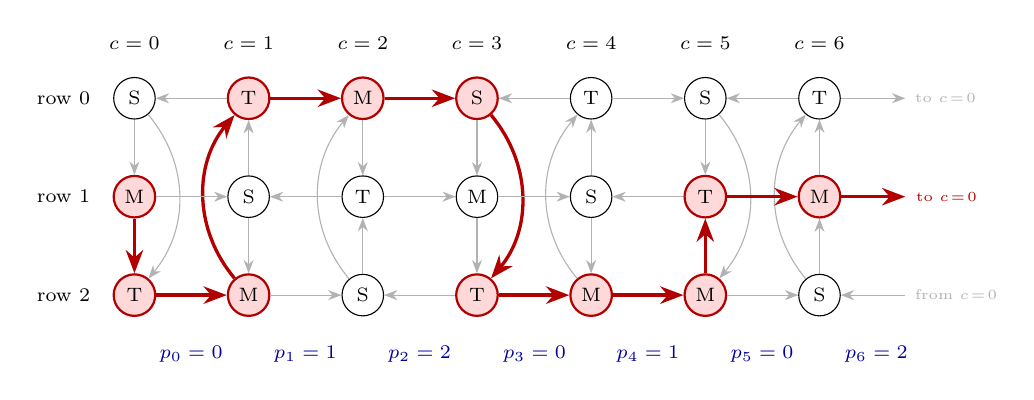
\begin{tikzpicture}[>=Stealth,v/.style={circle,draw,inner sep=1.2pt,minimum size=15pt,font=\scriptsize}]
\node[v] (v00) at (0.00,0.00) {S};
\node[v,fill=red!15,draw=red!70!black,thick] (v10) at (0.00,-1.25) {M};
\node[v,fill=red!15,draw=red!70!black,thick] (v20) at (0.00,-2.50) {T};
\node[font=\scriptsize] at (0.00,0.7) {$c=0$};
\node[font=\scriptsize,text=blue!60!black] at (0.72,-3.25) {$p_0=0$};
\node[v,fill=red!15,draw=red!70!black,thick] (v01) at (1.45,0.00) {T};
\node[v] (v11) at (1.45,-1.25) {S};
\node[v,fill=red!15,draw=red!70!black,thick] (v21) at (1.45,-2.50) {M};
\node[font=\scriptsize] at (1.45,0.7) {$c=1$};
\node[font=\scriptsize,text=blue!60!black] at (2.17,-3.25) {$p_1=1$};
\node[v,fill=red!15,draw=red!70!black,thick] (v02) at (2.90,0.00) {M};
\node[v] (v12) at (2.90,-1.25) {T};
\node[v] (v22) at (2.90,-2.50) {S};
\node[font=\scriptsize] at (2.90,0.7) {$c=2$};
\node[font=\scriptsize,text=blue!60!black] at (3.62,-3.25) {$p_2=2$};
\node[v,fill=red!15,draw=red!70!black,thick] (v03) at (4.35,0.00) {S};
\node[v] (v13) at (4.35,-1.25) {M};
\node[v,fill=red!15,draw=red!70!black,thick] (v23) at (4.35,-2.50) {T};
\node[font=\scriptsize] at (4.35,0.7) {$c=3$};
\node[font=\scriptsize,text=blue!60!black] at (5.08,-3.25) {$p_3=0$};
\node[v] (v04) at (5.80,0.00) {T};
\node[v] (v14) at (5.80,-1.25) {S};
\node[v,fill=red!15,draw=red!70!black,thick] (v24) at (5.80,-2.50) {M};
\node[font=\scriptsize] at (5.80,0.7) {$c=4$};
\node[font=\scriptsize,text=blue!60!black] at (6.52,-3.25) {$p_4=1$};
\node[v] (v05) at (7.25,0.00) {S};
\node[v,fill=red!15,draw=red!70!black,thick] (v15) at (7.25,-1.25) {T};
\node[v,fill=red!15,draw=red!70!black,thick] (v25) at (7.25,-2.50) {M};
\node[font=\scriptsize] at (7.25,0.7) {$c=5$};
\node[font=\scriptsize,text=blue!60!black] at (7.97,-3.25) {$p_5=0$};
\node[v] (v06) at (8.70,0.00) {T};
\node[v,fill=red!15,draw=red!70!black,thick] (v16) at (8.70,-1.25) {M};
\node[v] (v26) at (8.70,-2.50) {S};
\node[font=\scriptsize] at (8.70,0.7) {$c=6$};
\node[font=\scriptsize,text=blue!60!black] at (9.42,-3.25) {$p_6=2$};
\draw[->,gray!60] (v00) to (v10);
\draw[->,gray!60,bend left=40] (v00) to (v20);
\draw[->,red!70!black,very thick] (v10) to (v20);
\draw[->,gray!60] (v11) to (v21);
\draw[->,gray!60] (v11) to (v01);
\draw[->,red!70!black,very thick,bend left=40] (v21) to (v01);
\draw[->,gray!60,bend left=40] (v22) to (v02);
\draw[->,gray!60] (v22) to (v12);
\draw[->,gray!60] (v02) to (v12);
\draw[->,gray!60] (v03) to (v13);
\draw[->,red!70!black,very thick,bend left=40] (v03) to (v23);
\draw[->,gray!60] (v13) to (v23);
\draw[->,gray!60] (v14) to (v24);
\draw[->,gray!60] (v14) to (v04);
\draw[->,gray!60,bend left=40] (v24) to (v04);
\draw[->,gray!60,bend left=40] (v05) to (v25);
\draw[->,gray!60] (v05) to (v15);
\draw[->,red!70!black,very thick] (v25) to (v15);
\draw[->,gray!60] (v26) to (v16);
\draw[->,gray!60,bend left=40] (v26) to (v06);
\draw[->,gray!60] (v16) to (v06);
\draw[->,gray!60] (v01) -- (v00);
\draw[->,gray!60] (v10) -- (v11);
\draw[->,red!70!black,very thick] (v20) -- (v21);
\draw[->,red!70!black,very thick] (v01) -- (v02);
\draw[->,gray!60] (v12) -- (v11);
\draw[->,gray!60] (v21) -- (v22);
\draw[->,red!70!black,very thick] (v02) -- (v03);
\draw[->,gray!60] (v12) -- (v13);
\draw[->,gray!60] (v23) -- (v22);
\draw[->,gray!60] (v04) -- (v03);
\draw[->,gray!60] (v13) -- (v14);
\draw[->,red!70!black,very thick] (v23) -- (v24);
\draw[->,gray!60] (v04) -- (v05);
\draw[->,gray!60] (v15) -- (v14);
\draw[->,red!70!black,very thick] (v24) -- (v25);
\draw[->,gray!60] (v06) -- (v05);
\draw[->,red!70!black,very thick] (v15) -- (v16);
\draw[->,gray!60] (v25) -- (v26);
\draw[->,gray!60] (v06) -- (9.79,0.00) node[right,font=\tiny]{to $c\!=\!0$};
\draw[->,red!70!black,very thick] (v16) -- (9.79,-1.25) node[right,font=\tiny]{to $c\!=\!0$};
\draw[<-,gray!60] (v26) -- (9.79,-2.50) node[right,font=\tiny]{from $c\!=\!0$};
\node[font=\scriptsize] at (-0.90,0.00) {row 0};
\node[font=\scriptsize] at (-0.90,-1.25) {row 1};
\node[font=\scriptsize] at (-0.90,-2.50) {row 2};
\end{tikzpicture}}
\caption{$C_3\T C_7$, $p=(0,1,2,0,1,0,2)$: the odd induced directed cycle (length 11) built by
Rule A plus the gadget at $c=2$.}
\end{figure}

\begin{theorem}[if, computer-assisted]
For odd $k$, the 12 Latin orientations of $C_3\T C_{3k}$ are kernel-perfect.
\end{theorem}
\emph{How:} kernel existence is checked column by column by a 20-state automaton. Every
induced subdigraph of $C_3\T C_{3k}$ is a product of $k$ boolean ``block'' matrices, and has a
kernel iff the product has a nonzero trace. The set of all products is finite, so one
closure computation covers every $k$. It fails for even $k$ (e.g.\ $C_3\T C_6$).

\paragraph{Result.} For odd $n$: $C_3\T C_n$ has a kernel-perfect admissible orientation iff
$3\mid n$, then exactly 12. And $C_5\T C_5$ has none.

\begin{ponder}
(1) Why period 3? (Order-3 Latin squares.) Is there a hand proof that Latin lifts are
kernel-perfect, e.g.\ via Galvin's stable-matching argument?
(2) Why does it fail for even $k$?
(3) For $m\ge5$ the columns are 5-cycles, which can be oriented in more ways. Can the
encoding lemma be generalised to prove that no $C_m\T C_n$ with $m,n\ge5$ works?
\end{ponder}

\textbf{What this buys the paper:} both classical methods (Alon--Tarsi and kernels) provably
fail on most of the open case. That is the justification for a new method like your partner's.

\section{Our work: first steps toward \texorpdfstring{$m=5$}{m = 5}}

\paragraph{Edge deletion still works.} Every coefficient $c_w$ ($w$ off the cycle of $e$) is
nonzero for $C_5\T C_5$, $C_5\T C_7$, $C_5\T C_9$, $C_5\T C_{11}$, $C_7\T C_5$, $C_7\T C_7$.
For $C_5\T C_5$ and $C_5\T C_7$ this is exact (computed modulo a prime), so for these the
``edge with disjoint lists'' corollary is proved.

\paragraph{But the algebra gets harder.} Nonzero eigenvalues of the transfer matrix:
\begin{center}
\begin{tabular}{@{}lrl@{}}
\toprule
$m$ & column states & nonzero eigenvalues\\
\midrule
3 & 6 & $\pm i\sqrt3$\\
5 & 30 & 6 pairs $\pm i\lambda$\\
7 & 126 & 25 pairs $\pm i\lambda$\\
\bottomrule
\end{tabular}
\end{center}
A closed form like $T^3=-3T$ is hopeless for $m=5$. A computer-assisted proof for each fixed
$m$ is realistic: as $n\to\infty$ the largest pair dominates, so $c_w\ne0$ for $n\ge n_0$ once
its amplitude is nonzero; check $n<n_0$ directly.

\paragraph{Counterexample search.} A SAT loop proposes lists and refutes them with
colourings. $C_3\T C_5$, 4 colours: no bad assignment. $C_5\T C_5$: unfinished, too slow as
written.

\begin{ponder}
Case B of the $m=3$ proof needs a colouring of $C_3\T C_3$ from row-constant lists. For
$C_5\T C_n$, what replaces it? (Hint: $C_5\T C_3\cong C_3\T C_5$, which your partner's theorem
covers. Repeat its three columns as $X,Y,Z,Y,Z,\ldots$.)
\end{ponder}

\section{What remains, in order}

These are the research steps; everything else is writing. ``Done'' criteria are in italics.

\paragraph{A. Make the $m=3$ theorem airtight (required).}
\begin{enumerate}[nosep]
\item Get [P]. Verify Lemma 3.5 (propagation) line by line, plus everything it uses.
\emph{Done when we can prove $(\ast)$ ourselves.}
\item Verify the strip lemma computation ([P, Theorem 4], Steps 1--3).
\emph{Done when our own code reproduces $c_S$ for small $m$ and the derivation checks.}
\item Test $(\ast)$ and the full theorem on small cases by computer: exhaustive search for
bad assignments of $C_3\T C_5$, $C_3\T C_7$ with 5--6 colours, using the overlap restriction.
\emph{Done when no counterexample appears in feasible ranges.}
\end{enumerate}

\paragraph{B. Finish the kernel section (required, ours).}
\begin{enumerate}[nosep]
\item Learn both proofs in Section 5 well enough to present without notes.
\item Optional but valuable: a hand proof that Latin lifts are kernel-perfect for odd $k$.
\end{enumerate}

\paragraph{C. Extend to $m=5$ (what makes it a strong paper).} For $C_5\T C_n$, all odd $n$:
\begin{enumerate}[nosep]
\item Edge deletion for all odd $n$ (dominant eigenvalue + finite check).
\item Odd strip lemma for $C_5\T P_k$: define end multisets, compute $c_S$, find the analogue
of $s\not\equiv0$, prove nonvanishing.
\item Two-column extension for 5-cycle columns (replace the prism lemma). Odd cycles with
2-lists are colourable unless all lists are equal: the starting point.
\item Propagation $(\ast)$ for $m=5$ (depends on what [P]'s proof uses).
\item Case B via $C_3\T C_5$ (see the last Ponder box).
\item Assemble Cases A and B. \emph{Done when $C_5\T C_n$ is 3-choosable for all odd $n$.}
\end{enumerate}
In parallel: a faster counterexample search for $C_5\T C_5$ (symmetry breaking, better
solver). If one exists, the conjecture is false, which is an even bigger result.

\paragraph{D. General $m$ (stretch).} Once $m=5$ works, see which lemmas are uniform in $m$.

\paragraph{When is it enough for a good journal?}
\begin{itemize}[nosep]
\item \textbf{Minimum:} A + B. A verified proof for all $C_3\T C_n$ (an infinite family of an
open conjecture), plus a theorem explaining why the standard methods fail. Solid for a
combinatorics journal.
\item \textbf{Strong:} A + B + C. Two infinite families, and a method shown to generalise.
\item \textbf{Exceptional:} D, or a counterexample.
\end{itemize}

\end{document}
